\documentclass[handout, 11pt]{beamer}

\usepackage[english] {babel}                 % Idioma (és important a l'hora de separar una paraula a final de línia)
%%\ProvidesPackage{myStyle}

% Plantilla versió 2.6.1                                4 / 1 / 2017

 \usepackage{bbm}                                       % Permet fer \1
            %%% Nota: Si la plantilla no compila, comenta els dos packages anteriors.
 \usepackage[utf8]{inputenc}                            % Accents i símbols extranys
 \usepackage{amsfonts,amssymb}                          % Símbols matemàtics
 \usepackage{mathrsfs}                                  % Lletra cal·ligràfica (millor que \mathcal)
 \usepackage{amsmath}                                   % Mode matemàtic
\usepackage{amsthm}										% TheoremStyle
\usepackage{bookman}                                   % BarreroTimes
 \usepackage{verbatim}                                  % Verbatim + comentaris multilínia
 \usepackage{graphicx,subcaption}                       % Fotos i subfotos
 \usepackage[free-standing-units]{siunitx}              % Sistema internacional
 \usepackage[siunitx, american]{circuitikz}             % Circuits
 \usepackage{multicol}
 \usepackage{float}                                     % Posa les figures on toca
 \usepackage{anysize}                                   % Posa els marges
 \marginsize{2cm}{2cm}{1cm}{4cm}     % {L}{R}{U}{D}
 \usepackage{tikz-cd}                                   % Diagrames commutatius
 \usetikzlibrary{babel}                                 % Evita interferència entre tikz-cd i babel
%\usepackage{helvet}                                     % Estas dos lineas
%\renewcommand{\familydefault}{\sfdefault}               % ponen Arial
\usepackage[toc,page]{appendix}                         % for appendices
\usepackage{enumerate}					% enumerate options
\usepackage{hyperref}					%for hyperrefferences  (needed in bibliography
\usepackage[square,comma,numbers,sort&compress]{natbib} % bibliography stuff (see http://www.colorado.edu/physics/phys4610/phys4610_sp12/bibtex_guide.pdf)
\usepackage{xcolor} %Texto colores
%\usepackage{bm}						%for bold math symbols \pmb  PROBLEMATIC FOR BEAMER
\usepackage[nobreak=true]{mdframed}					% this is to frame theorems and definitions and figures
\usepackage{lmodern}
\usepackage{pst-func}
\usepackage{pst-ode,pst-plot}

\usepackage{pstricks}
%\usepackage{authblk}			% author affiliation PROBLEMATIC FOR BEAMER
%\usepackage{enumitem}
\usepackage{moreenum}
\usepackage{cleveref} % Clever referencing http://ctan.math.washington.edu/tex-archive/macros/latex/contrib/cleveref/cleveref.pdf

\setcounter{secnumdepth}{5}

\numberwithin{equation}{section}			% equation numbering
\setlength{\parskip}{1em}
\setlength\parindent{0cm}


\renewcommand\emph[1]{\textit{\textbf{#1}}}

%Conjunts importants
\def\NN{\mathbb N}   % Naturals
\def\ZZ{\mathbb Z}   % Enters
\def\QQ{\mathbb Q}   % Racionals
\def\RR{\mathbb R}   % Reals
\def\CC{\mathbb C}   % Complexos
\def\HH{\mathbb H}   % Quaternions, semiplà superior complex
\def\AA{\mathbb A}   % Espai afí en general
\def\EE{\mathbb E}   % Extensió d'un cos, esperança
\def\FF{\mathbb F}   % Cos primer, cos finit
\def\KK{\mathbb K}   % Cos en general
\def\PP{\mathbb P}   % Espai projectiu, nombres primers
\def\DD{\mathbb D}   % Disc unitat complex
\def\SS{\mathbb S}   % Esfera
\def\TT{\mathbb T}   % Tor (n-dimensional)
\def\XX{\mathbb X}   

\def\C{\mathcal C}                                      % Funcions contínues, derivables amb continuïtat
\def\D{\mathcal D}	%Deep networks
\def\F{\mathcal F}	%Deep networks
\def\G{\mathcal G}	% Graph
\def\S{\mathcal S}	% Shallow "

% Per escriure menys
\def\oo{\infty}                                         % Infinit
\def\P{\mathscr P}                                      % Conjunt potència
\def\A{\mathscr A}                                      % Àlgebra, sigma-àlgebra
\def\B{\mathscr B}                                      % Base
\def\T{\mathscr T}                                      % Topologia
%\def\L{\mathscr L}                                      % Espai d'homomorfismes, derivada de Lie
\def\O{\mathcal O}										% big O notation
\def\D{\mathscr D}                                      % Funcions derivables
\def\mm{\mathfrak M}                                    % Matrius
%\def\ss{\mathfrak S}                                    % Grup simètric
\def\aa{\mathfrak A}                                    % Grup alternat
\def\Re#1{\mathrm {Re}\left(#1\right)}              % Part real
\def\Im#1{\mathrm {Im}\left(#1\right)}              % Part imaginària
\def\1{\mathbbm{1}}                                     % Funció indicadora
\def\<{\langle}                                         % subespai/ideal/subgrup -
\def\>{\rangle}%                                          generat per, producte escalar
\def\sect{\mathsection}                                 % Secció
\def\pgph{\mathparagraph}                               % Fi de paràgraf
\def\qed{\hfill\square}                                 % Quadrat blanc de Q.E.D.
\def\defs{\stackrel{\tiny{\mbox{def}}}{=}}		% For definitions

%Calia
\def\phi{\varphi}       %%% Aquesta comanda inhabilita el "\phi" lleig
\def\eps{\varepsilon}   %\epsilon

\DeclareMathOperator*{\argmin}{arg\,min}                                 % Punt on s'assoleix el mínim
\DeclareMathOperator*{\argmax}{arg\,max}                                 % Punt on s'assoleix el màxim
\DeclareMathOperator*{\mex}{mex}                                         % Mínim ordinal exclòs
\DeclareMathOperator*{\sgn}{sgn}                                         % Signe
\DeclareMathOperator*{\im}{Im}                                           % Imatge
\DeclareMathOperator*{\Tr}{Tr}                                           % Traça
\DeclareMathOperator*{\Id}{Id}                                           % Identitat
\DeclareMathOperator*{\supp}{supp}                                       % Suport
\DeclareMathOperator*{\esup}{ess\,sup}                                   % Essential support
\DeclareMathOperator*{\Span}{span}                                       % Span
\DeclareMathOperator*{\prolim}{\underleftarrow{\rm{proj\,lim}}}          % Límit projectiu
\DeclareMathOperator*{\indlim}{\underrightarrow{\rm{ind\,lim}}}          % Límit inductiu

%Trigonometria bàsica
\DeclareMathOperator*{\tg}{tg}                          % tg(·)          = sin(·)/cos(·)
\DeclareMathOperator*{\cosec}{cosec}                    % cosec(·)       = 1/sin(·)
\DeclareMathOperator*{\cotg}{cotg}                      % cotg(·)        = cos(·)/sin(·)

\DeclareMathOperator*{\arctg}{arctg}
\DeclareMathOperator*{\arcsec}{arcsec}
\DeclareMathOperator*{\arccosec}{arccosec}
\DeclareMathOperator*{\arccotg}{arccotg}

\DeclareMathOperator*{\tgh}{tgh}                        % tgh(·)         = sinh(·)/cosh(·)
\DeclareMathOperator*{\sech}{sech}                      % sech(·)        = 1/cosh(·)
\DeclareMathOperator*{\cosech}{cosech}                  % cosech(·)      = 1/sinh(·)
\DeclareMathOperator*{\cotgh}{cotgh}                    % cotgh(·)       = cosh(·)/sinh(·)

\DeclareMathOperator*{\arcsinh}{arcsinh}
\DeclareMathOperator*{\arccosh}{arccosh}
\DeclareMathOperator*{\arctgh}{arctgh}
\DeclareMathOperator*{\arcsech}{arcsech}
\DeclareMathOperator*{\arccosech}{arccosech}
\DeclareMathOperator*{\arccotgh}{arccotgh}

% Operadors grans
\DeclareMathOperator*{\bigcomma}{\raisebox{0.9ex}{\Huge ,}}  % Comatori                    %% e.g. $\RR = \left\{\bigcomma\limits_{x\in\RR} x \right\}$
\DeclareMathOperator*{\bigtimes}{\text{\Large $\times$}}     % Cartesionatori              %% e.g. $\bigtimes\limits_{i\in B} A = A^B :=\{f:B\to A\}$
\DeclareMathOperator*{\bigvoid}{\text{\Large $\O$}}          % Concatenatori               %% e.g. $\bigvoid\limits_{i=1}^n \left(\sum\limits_{j_i=1}^n\right) 1 = n^n$
\DeclareMathOperator*{\bigequals}{\text{\Large $=$}}         % Igualatori                  %% e.g. $\bigequals\limits_{n=1}^\oo \sum\limits_{i=1}^n \dfrac1n$
\DeclareMathOperator*{\bigle}{\text{\Large $\le$}}           % Creixentatori               %% e.g. $0<\bigle\limits_{n=1}^\oo a_n<k\implies\exists\lim\limits_{n\to\oo}a_n\leq k$
\DeclareMathOperator*{\bigge}{\text{\Large $\ge$}}           % Decreixentatori
\DeclareMathOperator*{\bigless}{\text{\Large $<$}}           % Creixentatori estricte
\DeclareMathOperator*{\biggreater}{\text{\Large $>$}}        % Decreixentatori estricte
\DeclareMathOperator*{\bigsse}{\text{\Large $\sse$}}         % Inclusionatori              %% e.g. $\O\sse\bigsse\limits_{n=1}^\oo (-n,n)\sse\R$
\DeclareMathOperator*{\bigspse}{\text{\Large $\spse$}}       % Antiinclusionatori
\DeclareMathOperator*{\bigsss}{\text{\Large $\sss$}}         % Inclusionatori estricte
\DeclareMathOperator*{\bigssne}{\text{\Large $\ssne$}}       % Inclusionatori estricte
\DeclareMathOperator*{\bigssps}{\text{\Large $\ssps$}}       % Antiinclusionatori estricte
\DeclareMathOperator*{\bigspsne}{\text{\Large $\spsne$}}     % Antiinclusionatori estricte
\DeclareMathOperator*{\bigni}{\text{\Large $\ni$}}           % Contenatori                 %% e.g. $\nexists\bigni\limits_{i=0}^\oo A_i$
\DeclareMathOperator*{\bigin}{\text{\Large $\in$}}           % Pertanyatori
\DeclareMathOperator*{\bigo}{\bigcirc}                       % Compositori                 %% e.g. $\bigequals\limits_{x\in\R}\left(\bigo\limits_{i=1}^\oo \cos\right) (x)$
\DeclareMathOperator*{\bigfrac}{\raisebox{-.5ex}{\Large K}}  % K-atori                     %% e.g. $\bigfrac\limits_{i=1}^\oo(b_i:c_i):=\cfrac{b_1}{c_1+\cfrac{b_2}{c_2+\ddots}}$
            %%% Nota: El sumadirectori (\bigoplus), els dos uniodisjuntatoris (\bigsqcup, \biguplus) i el tensionatori (\bigotimes) ja estan implementats per defecte.
\newcommand\restr[2]{{% we make the whole thing an ordinary symbol    		%restriccions de funcions
  \left.\kern-\nulldelimiterspace % automatically resize the bar with \right
  #1 % the function
  \vphantom{\big|} % pretend it's a little taller at normal size
  \right|_{#2} % this is the delimiter
  }}




\usetheme{CambridgeUS}
\usepackage{color}
\usepackage{amssymb,mathtools, amsmath, amsfonts, amsthm}
\usepackage{graphicx}
\usepackage{float}
%\usepackage{hyperref}
%\usepackage{enumerate}
%\usepackage{enumitem}
\usepackage{chngcntr}
%\usepackage{cleveref}
\usepackage{pdfpages}
\setbeamertemplate{itemize items}[circle]

\newcommand{\cc}{\mathfrak{c}}
\newcommand{\Z}{\mathbb{Z}}
\newcommand{\CC}{\mathbb{C}}
\newcommand{\Q}{\mathbb{Q}}
\newcommand{\R}{\mathbb{R}}
\newcommand{\N}{\mathbb{N}}
\newcommand{\Hc}{\mathcal{H}}
\newcommand{\Lan}{\mathcal{L}}
\newcommand{\Ln}{\lim\limits_{n\to \infty}}
\newcommand{\clist}{\mathfrak{c}_{1}, \cdots, \mathfrak{c}_m}
\newcommand{\morph}[1]{\stackrel{#1}{\simeq}}
\newcommand{\vlst}[2]{#1_1,\dots, #1_{#2}}
\newcommand{\gnp}{G(n,\beta_1/n^{a_1-1}, \dots,\beta_l/n^{a_l-1})}


\setbeamertemplate{itemize items}[circle]

\AtBeginSection[]
{
	\begin{frame}{Contents}
	\tableofcontents[currentsection]
	\end{frame}
}

\title[First Order Logic of Sparse Random Hyper-Graphs]{First Order
	Logic of Sparse Random Hyper-Graphs}

\author{L\'azaro Alberto Larrauri Borroto \\ 
	Supervisor: Marc Noy Serrano}

\date\today


\begin{document}
	\frame{\titlepage}
	\frame{\tableofcontents}


	\section{First Order Logic of Sparse Graphs}
	\begin{frame}{The first order language of graphs.}
		\begin{columns}
			\begin{column}{0.55\textwidth}
				\begin{itemize}
					\item Variables $x_1, \dots, x_n, \dots$
					\item Connectives $\wedge, \vee$, equality symbol $=$,
					and negation symbol $\neg$.
					\item Quantifiers $\forall, \exists$.
					\item A binary relation symbol $R$
				\end{itemize}
			\end{column}
			\begin{column}{0.45\textwidth}
				\begin{itemize}
					\item Vertices.
					\item ``And", ``or", ``equals", ``not".
					\item ``For all", ``there exists".
					\item Edges $x\sim y$. 
				\end{itemize}
			\end{column}
		\end{columns}
		~\\
		\[ \forall x_1,x_2 \, R(x_1,x_2) \implies \exists x_3 (\,
		\neg(x_3=x_1)\wedge \neg(x_3=x_2) \wedge R(x_1, x_3))\]
	\end{frame}

	\begin{frame}{The binomial model}
	The binomial model of random graphs $G(n,p)$ is a discrete probability space where 
	we assign to each graph $G=([n],E)$ the probability
	\[\mathrm{Pr}(G)= p^{|E|}\cdot (1-p)^{\binom{n}{2}- |E| }. \]
	\end{frame}

	\begin{frame}{Lynch's theorem}
	\begin{theorem}[Lynch, 1992]
		Let $\varphi$ be a sentence in the F.O. language of graphs. 
		Then the map $\mathrm{F}_\varphi: [0,\infty) \rightarrow \R$ given by 
		\[\mathrm{F}_\varphi(\beta)=\Ln \mathrm{Pr}(\, G(n,\beta/n)\models \varphi \,) \]
		is well defined and admits an analytic extension to $\CC$.
	\end{theorem}
	\end{frame}
	
	\begin{frame}{Overview of the proof}
	Some properties of $G(n,\beta/n)$:
	\\~\\
	\begin{itemize}
		\item The number of cycles of 
		length $3,4\dots, r$
		are asymptotically distributed like independent Poisson 
		variables.
		\item Small cycles are a.a.s far away.
		\item Fixed vertices are a.a.s far away.
		\item The ball of a given radius centered in fixed
		vertex is a.a.s a tree. Any tree occurs with a positive 
		probability.
	\end{itemize}
	
	\end{frame}

	\begin{frame}{Overview of the proof}
	For each fixed quantifier rank $k$:
	\\~\\
		\begin{itemize}
			\item[(1)]	It is given a finite classification of "small" uni-cycles.
			\item[(2)]  It is shown that the rank $k$ type of random graph $G$
			 in $G(n,\beta/n)$ a.a.s depends exclusively on the number of "small" uni-cycles
			 belonging to each class. 
			\item[(3)] The asymptotic distribution of those quantities is obtained. 
		\end{itemize}
		
	\end{frame}
	\section{General relational structures}
	\begin{frame}{Edge sets}
		\begin{definition} Fix
			\begin{itemize}
				\item natural numbers $n,a\in \N$, with $a\geq 2$
				\item a subgroup of the symmetric group $\Phi \leq S_a$
				\item and a subset of pairs $A\subset ([a]\times [a]) \setminus \Delta_a$.
			\end{itemize}
		The \textbf{total edge set} $\mathcal{H}_{(a,\Phi, A)}(n)$ of size $a$, 
		symmetry group $\Phi$ and
		restrictions $A$, on $n$ elements is the set
		\[ \mathcal{H}_{(a,\Phi, A)}(n)= ([n]^a/\Phi) \, \,
		\setminus R, \]
		where
		\[ R = \{\,  [x_1, \dots,x_a] \in [n]^a/\Phi  \, \, 
		| \, \, x_i=x_j \, \text{for some } (i,j)\in A \} \] 
		\end{definition}
	\end{frame}
	\begin{frame}{Graphs}
		\begin{definition}
			An (hyper)-graph $([n], H_1,\dots, H_c)$ with edge colors 
			$1,\dots, c$, sizes $a_1,\dots,a_c$, 
			symmetry groups $\Phi_1,\dots,\Phi_c$ and 
			restrictions $A_1,\dots,A_c$ consists of 
			\begin{itemize}
				\item The vertex set $[n]$ for some natural number $n$.
				\item For $i=1,\dots,c$, a ``colored" edge set $H_i\subseteq \mathcal{H}_{(a_i,\Phi_i,A_i)}(n)$ whose elements 
				have color $i$.
			\end{itemize}
		\end{definition}
	\end{frame}
	 
	\begin{frame}{The first order language}
	Consider the first order purely relational language $\mathcal{L}$ whose signature consists of the relation symbols
	$R_1,\dots, R_c$ with arities $a_1,\dots,a_c$. \\~ \par
	
	A graph $G=([n],H_1,\dots, H_c)$ is a $\mathcal{L}$-structure in the following way:
	\begin{itemize}
		\item The universe of $G$ is its vertex set, $[n]$.
		\item For each $1\leq i \leq c$, 
		\[(x_1,\dots,x_{a_i})\in R_i^G \iff [x_1,\dots, x_{a_i}]\in H_i. \] 
	\end{itemize}
%		\begin{columns}
%			\begin{column}{0.55\textwidth}
%				\begin{itemize}
%					\item Variables $x_1, \dots, x_n, \dots$
%					\item Connectives $\wedge, \vee$, equality symbol $=$,
%					and negation symbol $\neg$.
%					\item Quantifiers $\forall, \exists$.
%					\item For each $1\leq i \leq c$ a relation symbol $R_i$ with arity $a_i$.
%				\end{itemize}
%			\end{column}
%			\begin{column}{0.45\textwidth}
%				\begin{itemize}
%					\item Vertices.
%					\item ``And", ``or", ``equals", ``not".
%					\item ``For all", ``there exists".
%					\item $i$-colored edges \\
%					$[x_1,\dots,x_{a_i}]$. 
%				\end{itemize}
%			\end{column}
%		\end{columns}
	\end{frame}

	\begin{frame}{The first order language}
		By definition, a graph $G=([n],H_1,\dots, H_n)$ satisfies, for each $1\leq i \leq c$:
		\vspace{0.5 em}
		\begin{itemize}
			\item Symmetry formulas:
			\[ S_g: =\big( R_i(x_1\dots,x_{a_i})\iff R_i(x_{g(1)}\dots,x_{g(a_i)})\big) ,\]
			where $g$ is an element from $\Phi_i$.
			\item Anti-reflexivity formulas:
			\[A_{i,(j,l)}:=\big(R_i(x_1\dots,x_{a_i})\implies 
			\neg(x_j= x_l)\big),\]
			where $(j,l)\in A_i$.
		\end{itemize}
		
	\end{frame}
	 
	\begin{frame}{The random model}

	The random model $HG(n,p_1,\dots, p_c)$ is a discrete probability space where for each graph 
	$G=([n],H_1,\dots,H_c)$,
	\[ \mathrm{Pr}(G)=\prod_{i=1}^{c} p_i^{|H_i|}\cdot (1-p_i)^{|\mathcal{H}_{(a_i,\Phi_i,A_i)}(n)|-|H_i|} . \]
	We consider the case where for each $1\leq i \leq c$,  $p_i(n)=\beta_i/n^{a_i-1}$.
	\\~\\ 
	Let $\beta=(\beta_1,\dots, \beta_c)\in [0,\infty)^c$. We abbreviate
	\[HG(n,p(n,\beta)):= HG(n,\beta_1/n^{a_1-1},\dots, \beta_c/n^{a_c-1}). \]
	
	\end{frame}
	
	\begin{frame}{The theorem}
		We want to prove the following
		
		\begin{theorem} Let $\varphi$ be a first order sentence in $\mathcal{L}$.
			Then the map $\mathrm{F}:[0,\infty)^c\rightarrow \R$ given by
			\[ \mathrm{F}(\beta_1,\dots, \beta_c)= \Ln 
			\mathrm{Pr}(HG(n,p(n,\beta))\models \varphi )
			\]
			is well defined and admits an analytic extension to $\CC^c$. 
		\end{theorem}
		
	\end{frame}
	
	\begin{frame}{Distance and paths}
		Given any graph $G$, we define the following distance over its vertex-set:
			
			\begin{equation*}d(x,y)= \min_{\substack{H \leq G\\ 
					H \text{ connected }\\
					x,y\in V(H)}} \big(|V(H)| - 1 \big), \, \, \text{ or } \infty \text{ if }
				x,y \text{ are not connected.}
			\end{equation*}
		
		\begin{definition} 
			A path between two vertices $x,y$ in a graph $G$ is
			a connected subgraph $H\leq G$ containing both $x,y$ whose
			number of vertices is minimum. 
		\end{definition}
		
	\end{frame}
	\begin{frame}{Likelihood, trees, cycles and clusters} 
		\begin{definition}
			The likelihood $L(G)$ of a graph $G=(V,H_1,\dots,H_c)$ is
			the number
			\[ |V(G)| - \sum_{i=1}^c |H_i|(a_i-1).\]
		\end{definition}
	~\\
	\end{frame}

	\begin{frame}{Likelihood, trees, cycles and clusters} 
	\begin{itemize}
		\item A tree is a connected graph with likelihood $1$.
		\vspace*{0.5 em}
	\end{itemize}
	
	\begin{center}
		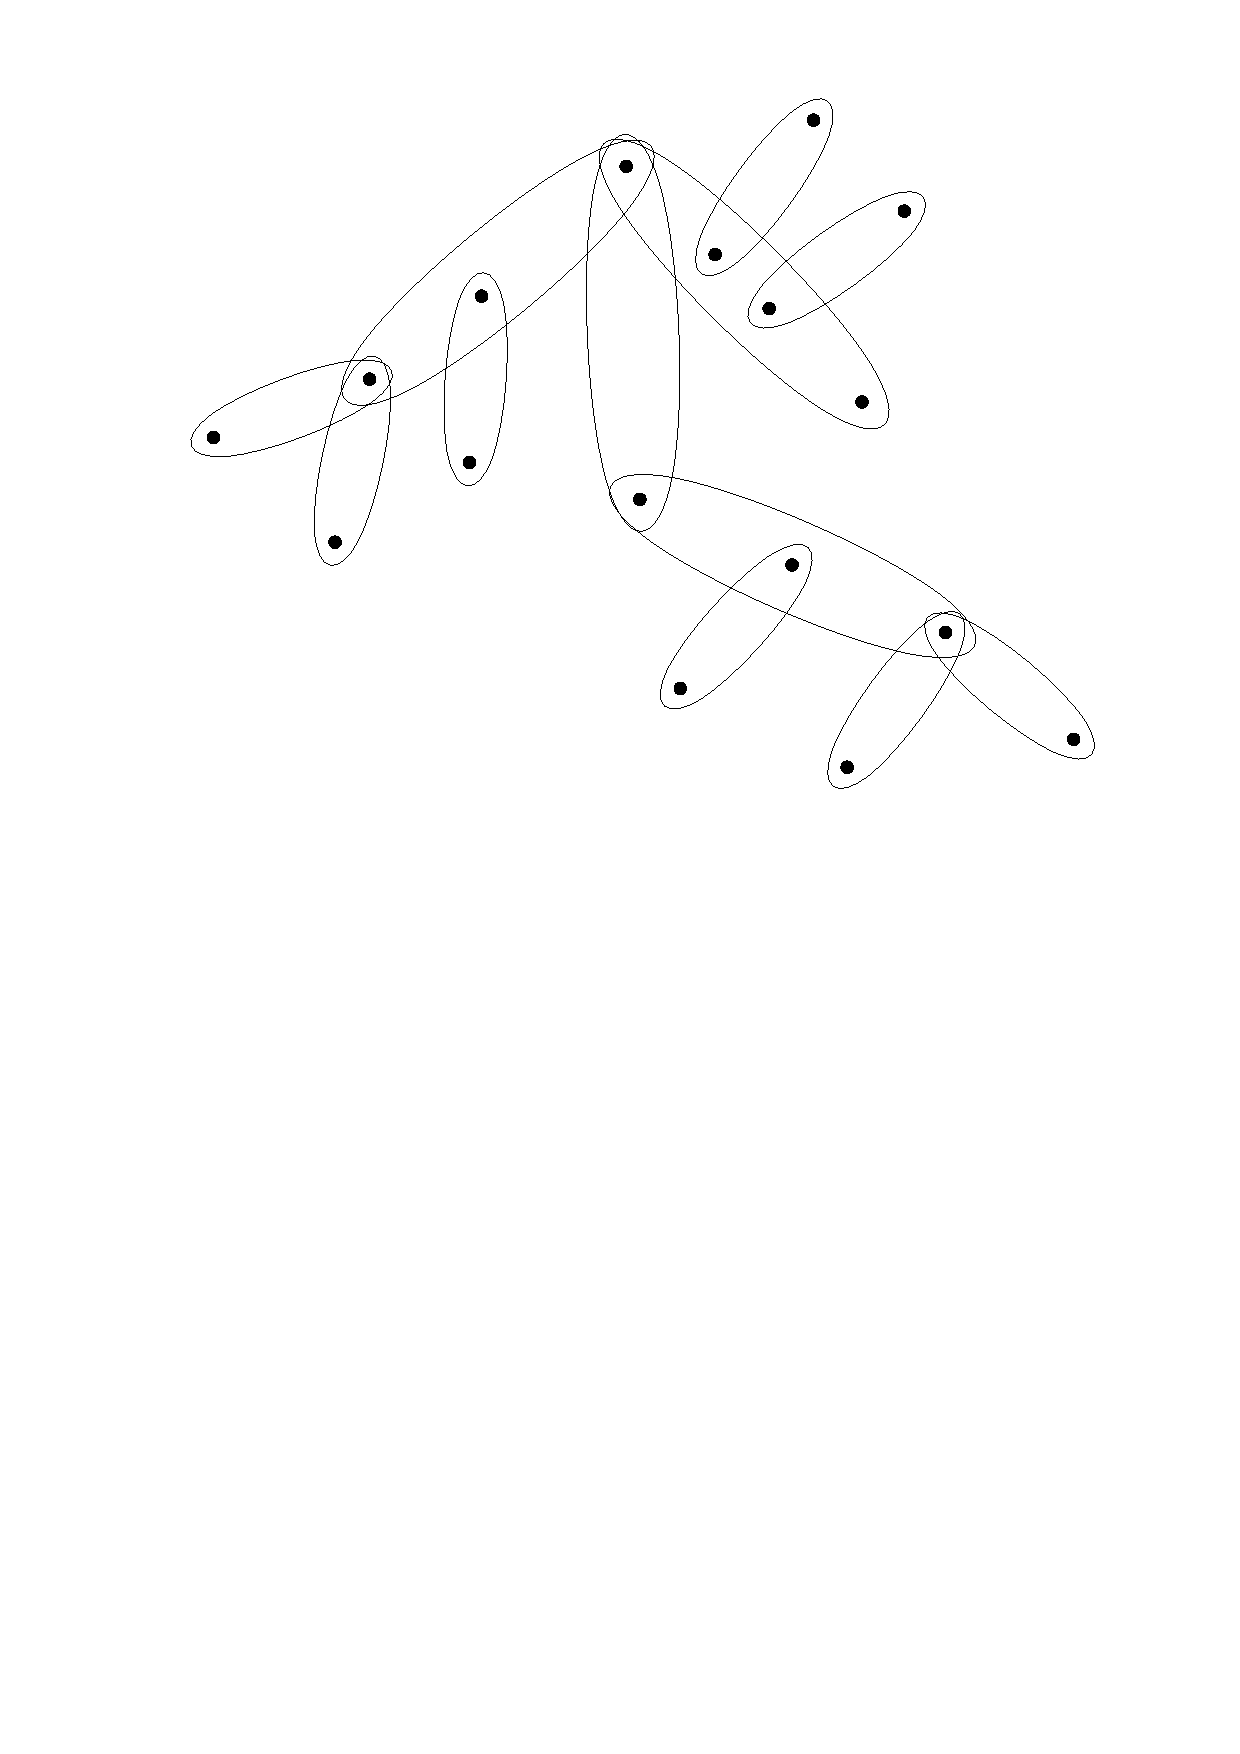
\includegraphics[width=0.7\linewidth]{Tree.pdf}
	\end{center}
	\end{frame}
	
	\begin{frame}{Likelihood, trees, cycles and clusters} 
		\begin{itemize}
			\item An unicycle is a connected graph with likelihood $0$.
			A cycle is a minimal unicycle.
		\end{itemize}
		\begin{center}
			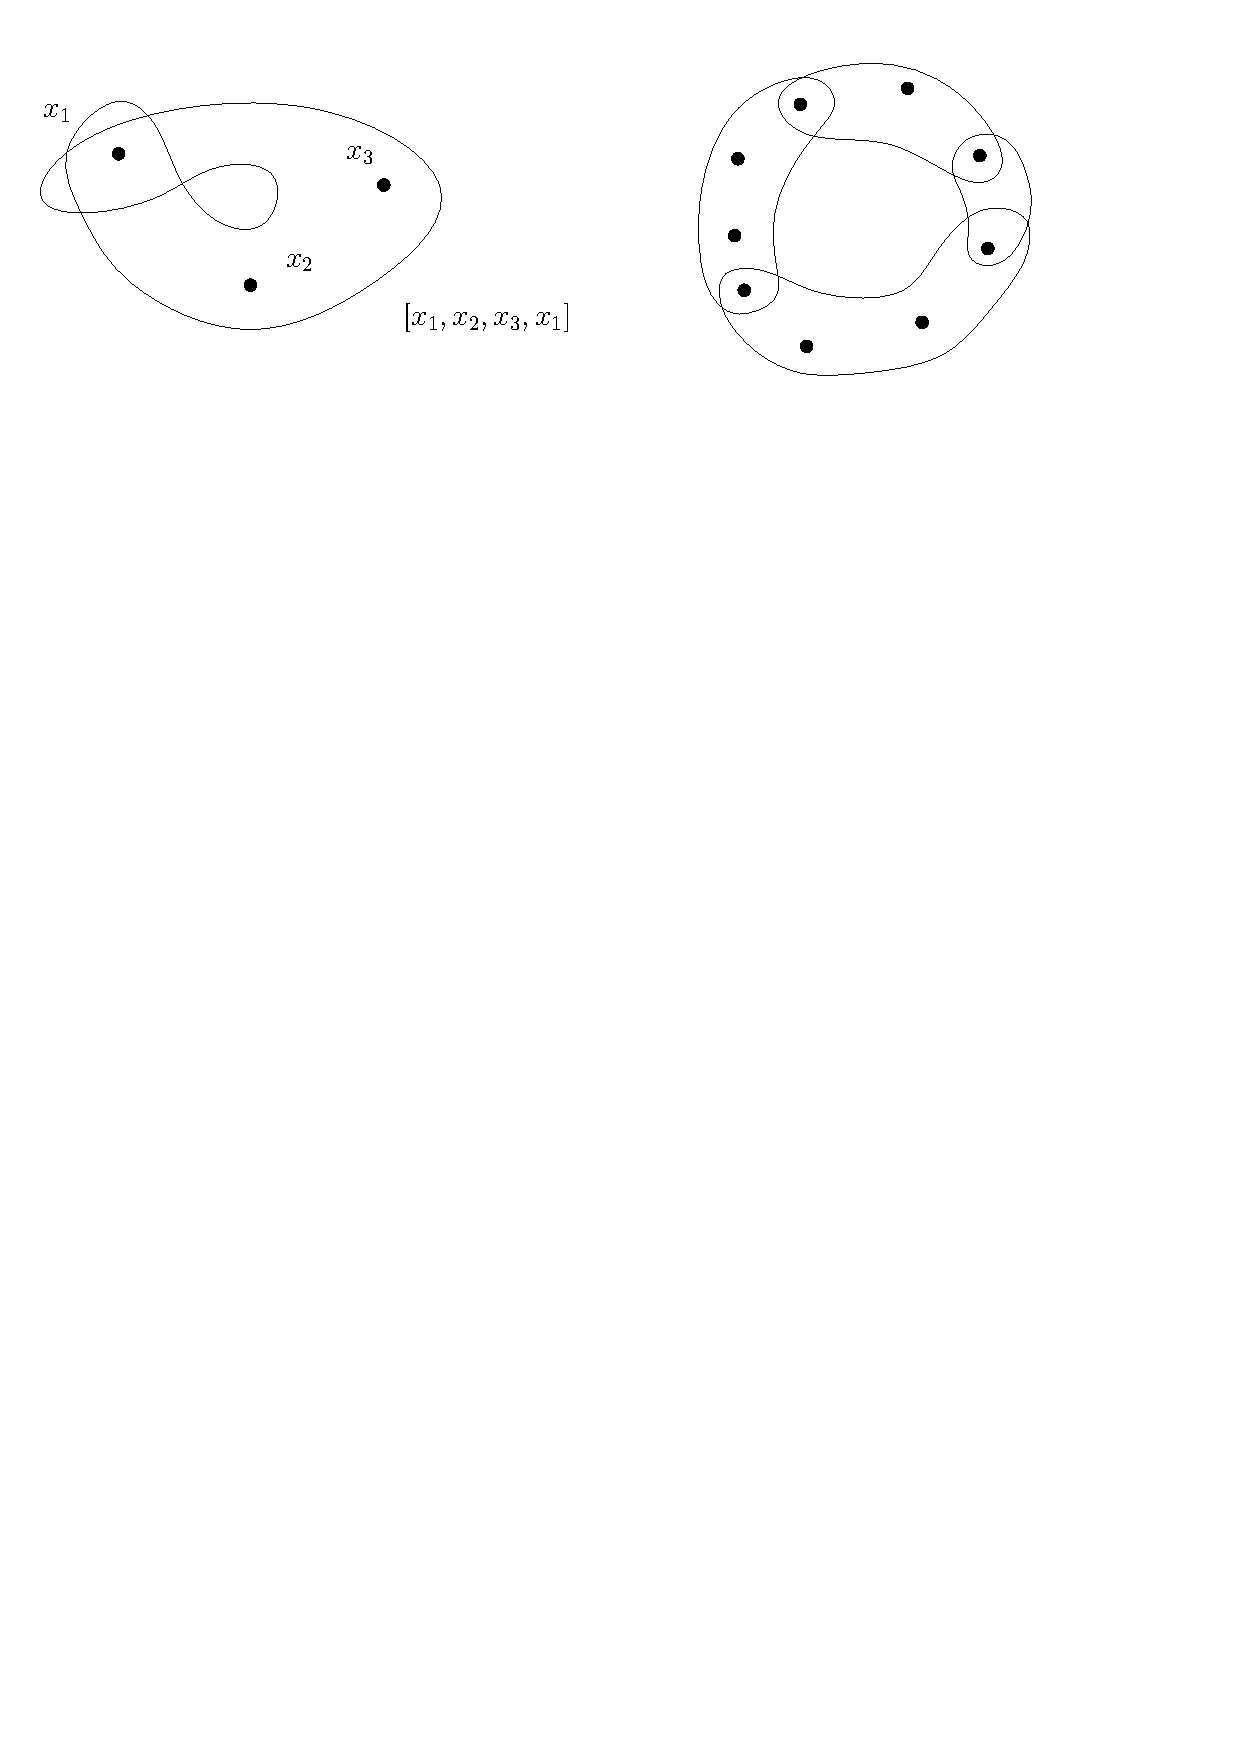
\includegraphics[width=0.9\linewidth]{Cycles.pdf}
		\end{center}
	\end{frame}

	\begin{frame}{Likelihood, trees, cycles and clusters}
		\begin{itemize}
			\item A cluster is a graph $G$ with $L(G)\leq 0$ such 
			that $L(H)>L(G)$\\ for any subgraph $H\leq G$.
		\end{itemize}
	\begin{center}
		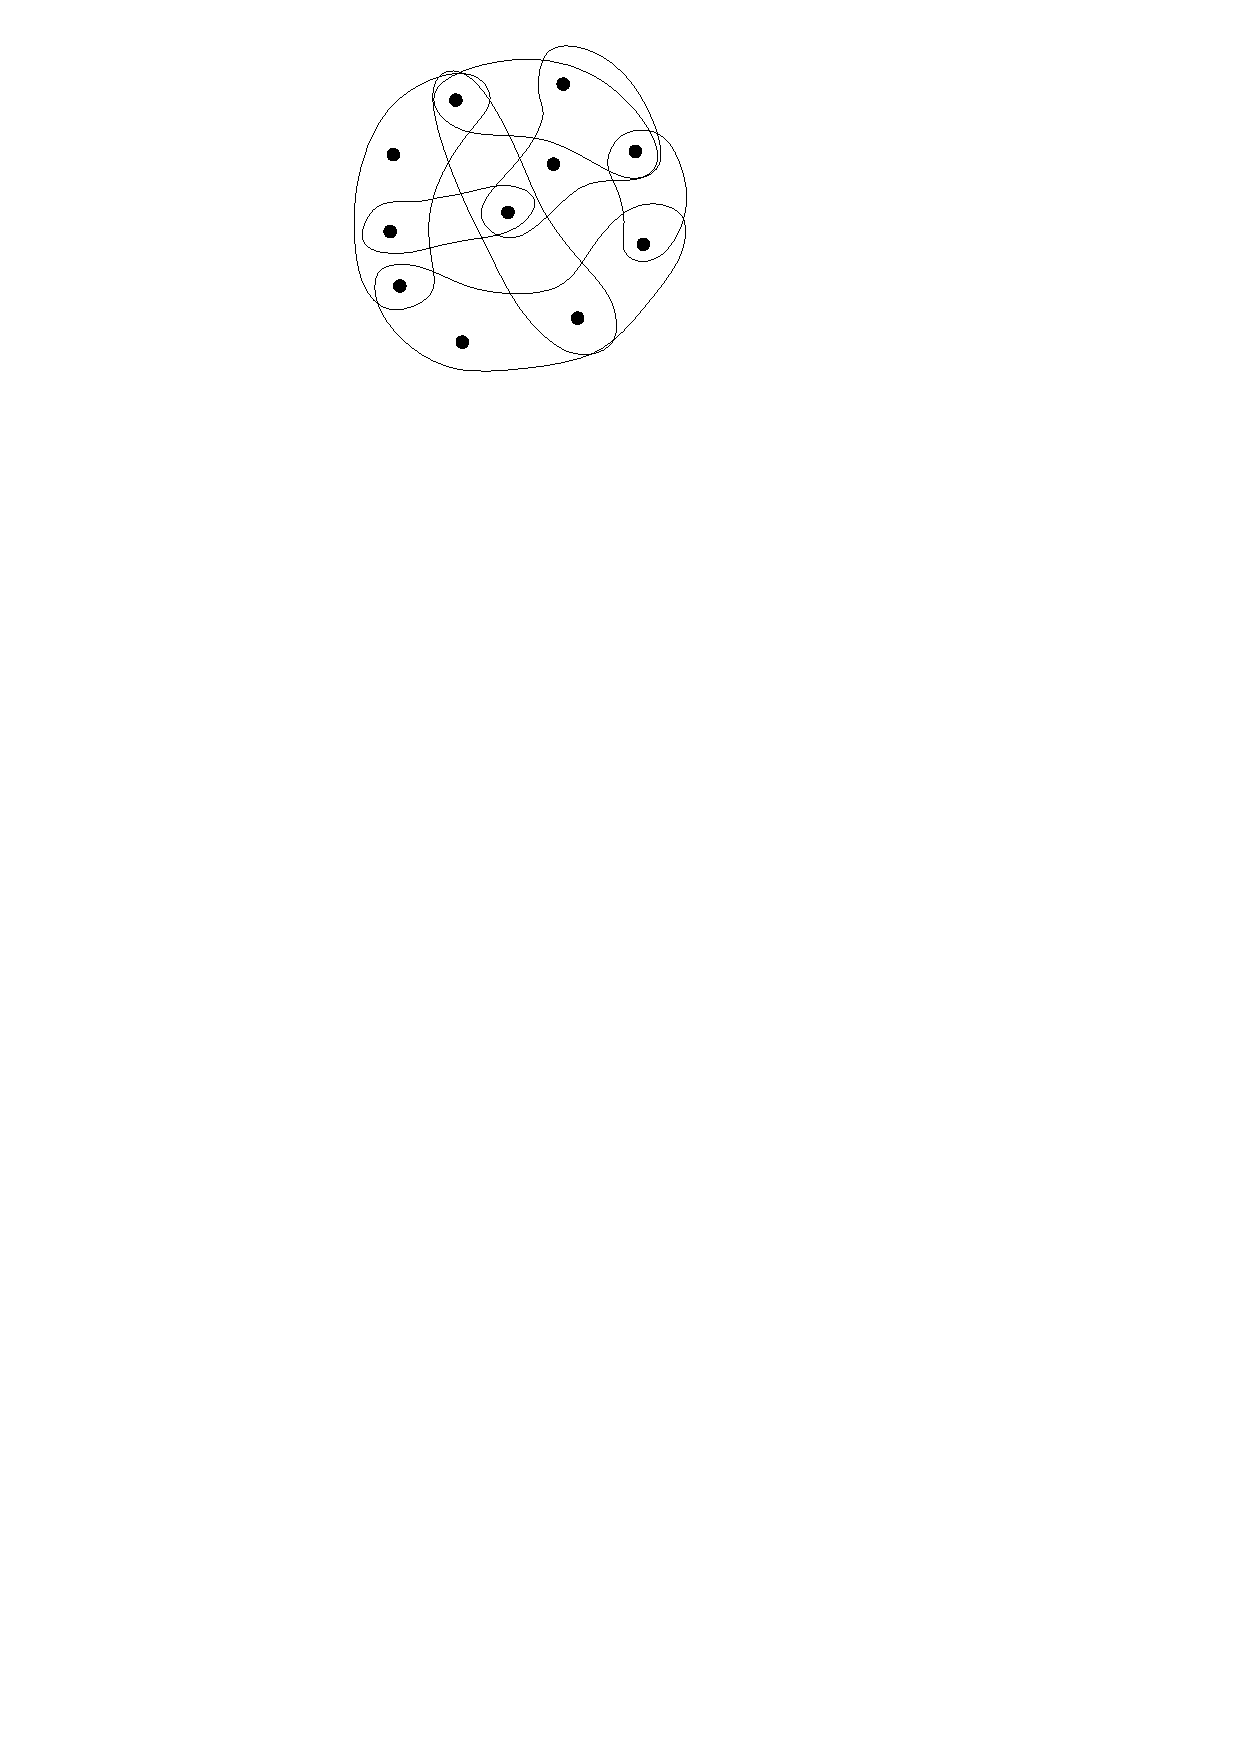
\includegraphics[width=0.4\linewidth]{Cluster.pdf}
	\end{center}
	\end{frame}
	
	\begin{frame}{The $k$-morphism relation over trees.}
		A rooted $(T,x)$ is a tree $T$ together with a distinguished vertex
		$x\in V(T)$.\par
		\[Tree(y, T) = (T[X], y),\]
		\[\text{where } \, X=\{ z\in V(T) \, | \, d(x,z)=d(x,y)+d(y,z)\}.\]~\\
		The root of an edge $e\in H(T)$ in a rooted tree 
		$(T,x)$ is the vertex $y\in e$ such that $d(x,y)=d(x,e)$.\\~\\
		The radius of an edge $e\in H(T)$ is 
		\[\max_{\substack{y\in e \\ y \text{ not the root of } e}} r(Tree(y,T)). \]
		
	\end{frame}

	\begin{frame}{The $k$-morphism relation over trees.}
		Fix $k\in \N$.\\
		We define the $k$-morphism relation over rooted trees of the same radius
		inductively as follows:
		
		\begin{itemize}
			\item If $r(T_1)=r(T_2)=0$ then $T_1\morph{k} T_2$.
		\end{itemize}
	\end{frame}

	\begin{frame}{The $k$-morphism relation over trees.}
		For $r>0$:
			\begin{itemize}
				\item  First we
				define the type of a en edge with radius less than $r$:
				
			\end{itemize}
		\begin{center}
			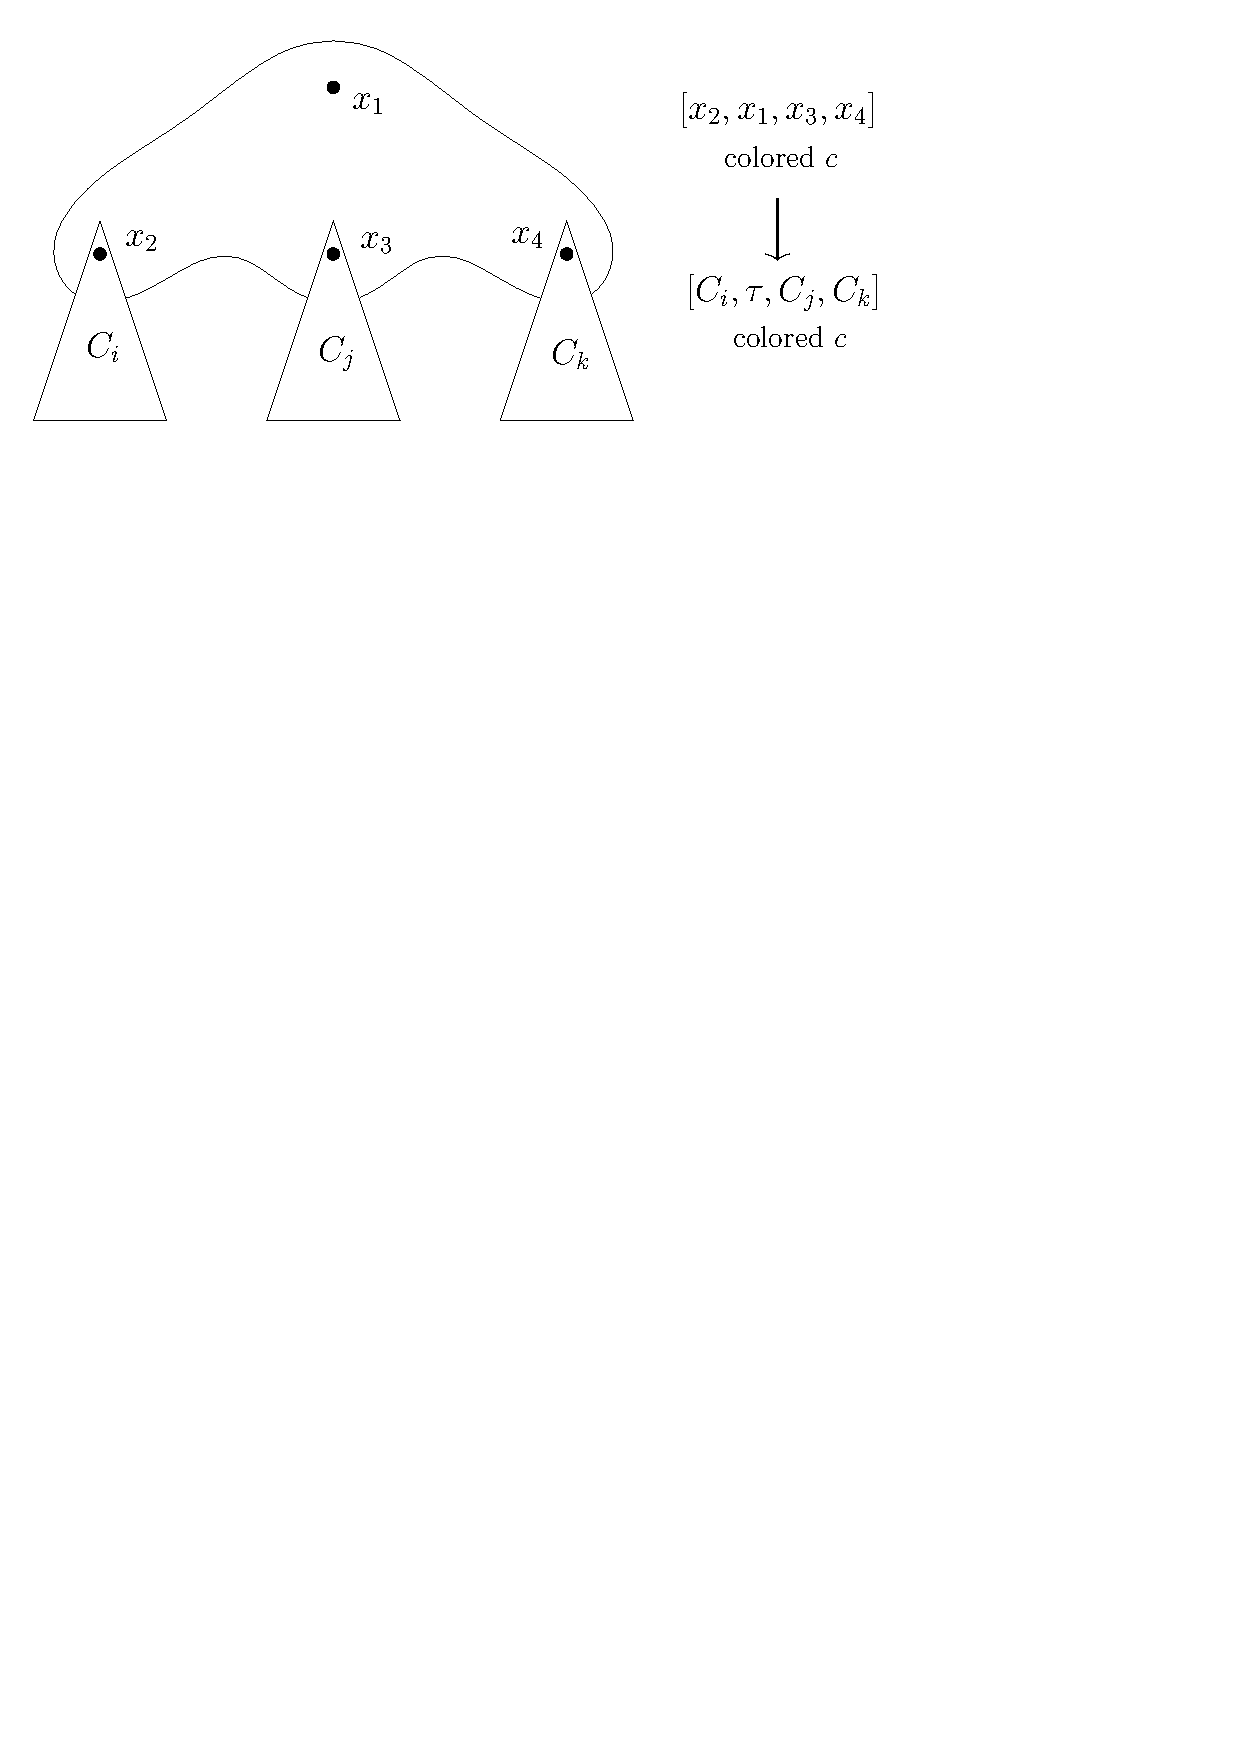
\includegraphics[width=0.8\linewidth]{Edgetype.pdf}
		\end{center}
	\end{frame}

	\begin{frame}{The $k$-morphism relation over trees.}
		\begin{itemize}
		\item If $r(T_1)=r(T_2)=r$ we say that $T_1\morph{K}T_2$ if
		for any edge $k$-type $E$ of radius less than $r$ either:
		\begin{itemize}
			\vspace{0.2 em}
			\item the number of initial edges in $T_1$ and $T_2$ of $k$-type $E$ 
			is the same, or
			\vspace{0.2 em}
			\item both $T_1$ and $T_2$ contain no less than $k+1$
			initial edges of $k$-type $E$. 
		\end{itemize}
		\begin{center}
			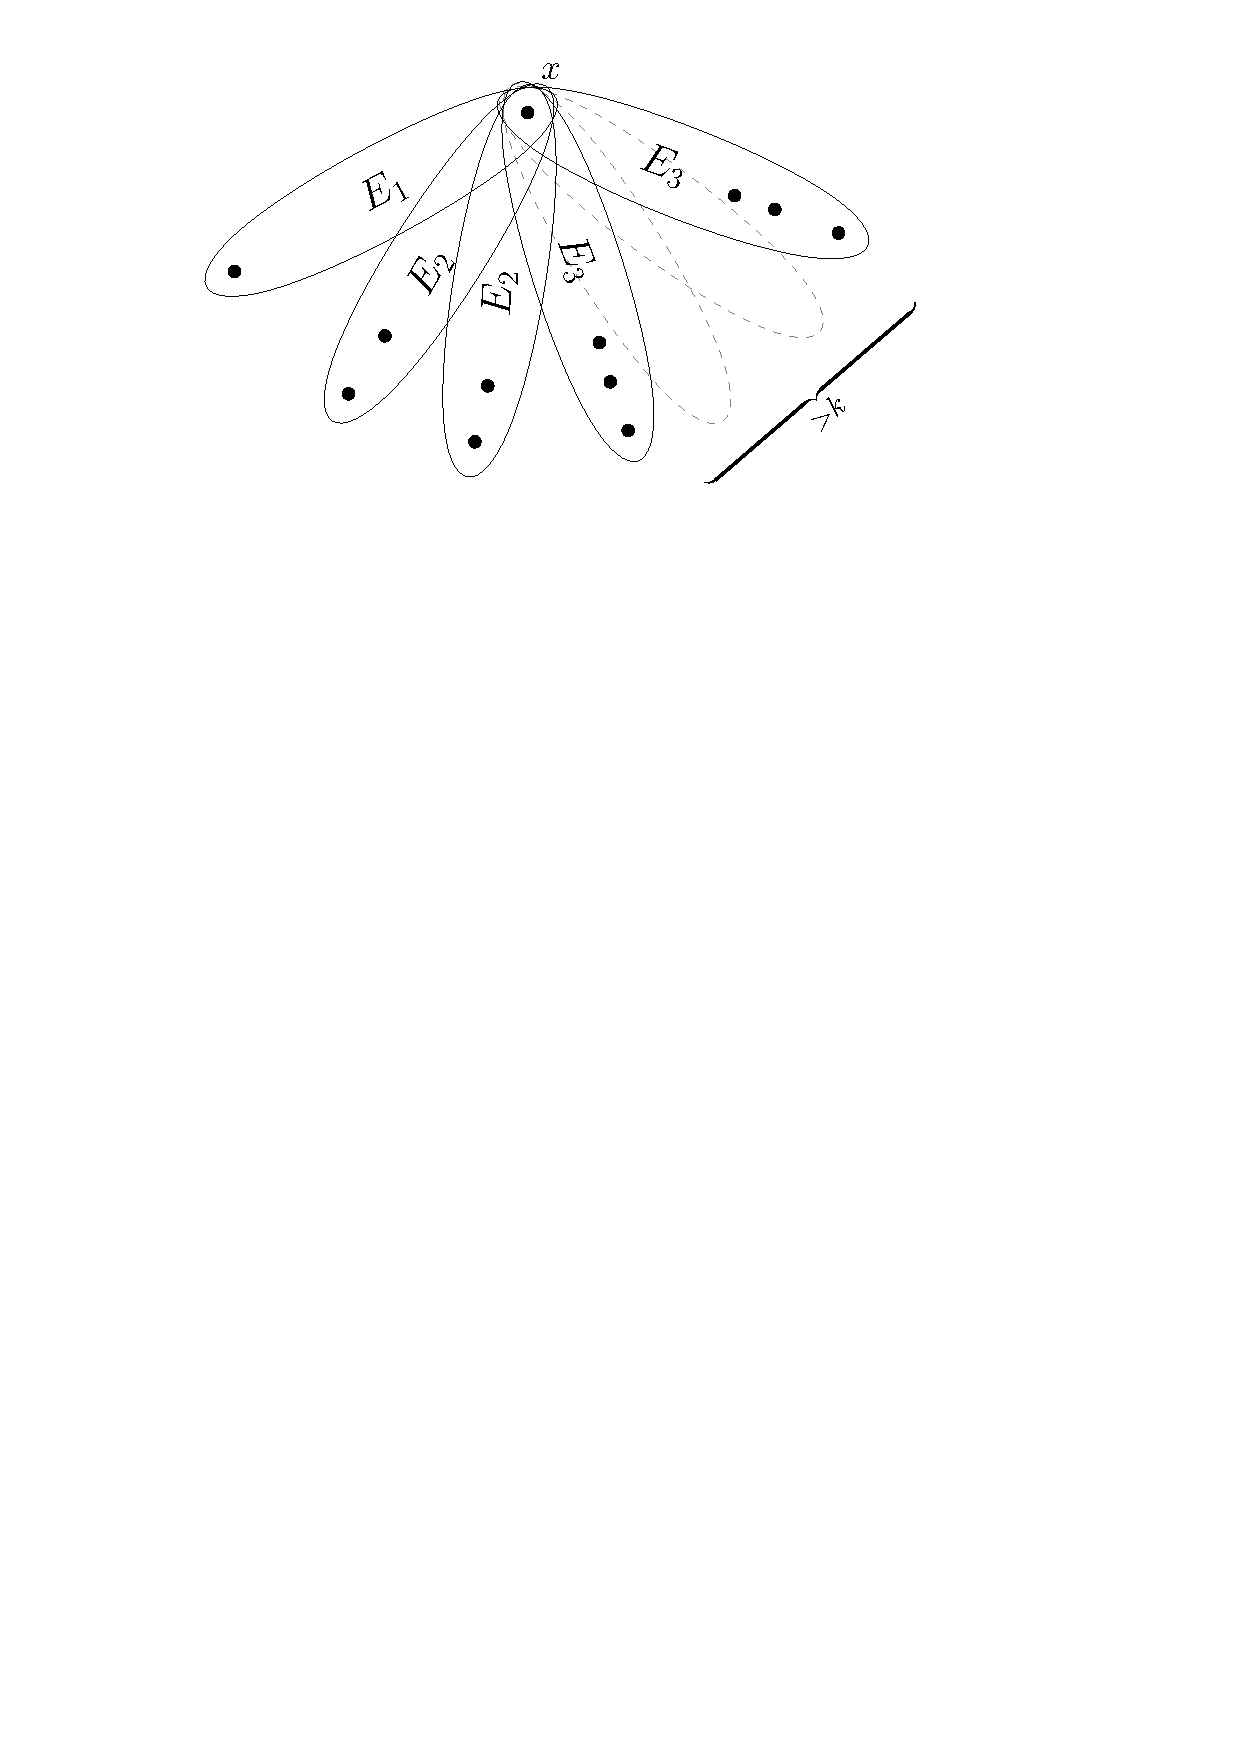
\includegraphics[width=0.7\linewidth]{Try.pdf}
		\end{center}
			
		\end{itemize}
	
		
	\end{frame}



\end{document}